\section{Durchführung}
Der Versuchsaufbau zur experimentellen Bestimmung der effektiven Masse von Leitungselektronen mittels Faraday-Effekt ist in \autoref{fig:aufbau} dargestellt.
Die Galliumarsenid-Probe ist transparent für Licht im Infrarotbereich.
\begin{figure}
    \centering
    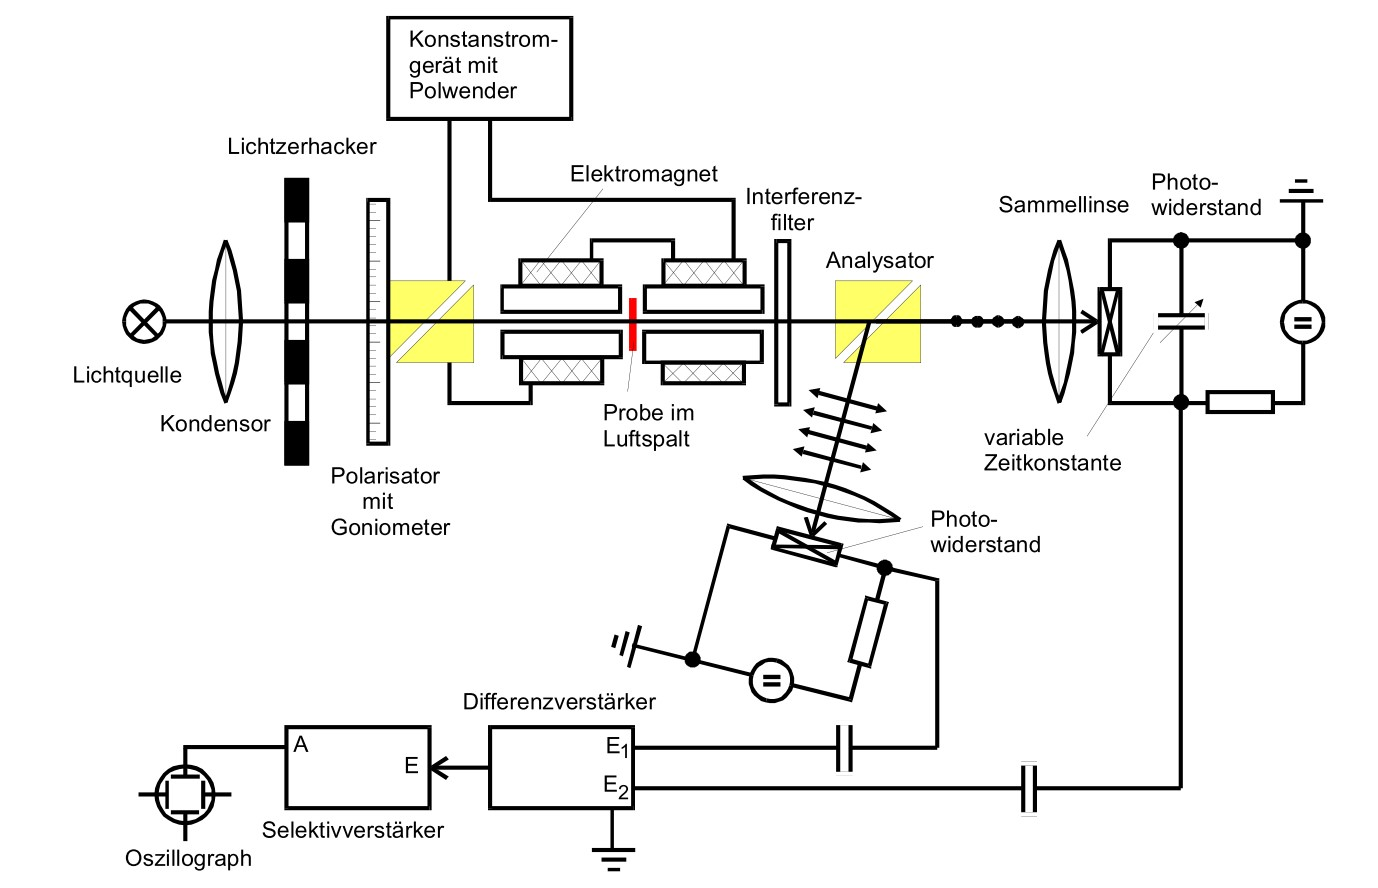
\includegraphics[width=0.8\textwidth]{figure/aufbau.jpg}
    \caption{Schematische Darstellung des Versuchaufbaus zur Bestimmung der effektiven Masse von Leitungselektronen mittel Faraday-Rotation. \cite{anleitung}}
    \label{fig:aufbau}
\end{figure}
Eine Halogen-Lampe emittiert Licht im sichtbaren bis Infrarot-Bereich.
Mithilfe einer Linse (Kondensor) wird der Lichtstrahl parallelisiert und auf den Lichtzerhacker abgebildet.
Als Lichtzerhacker wird eine rotierende Scheibe mit Aussparungen bezeichnet.
Dieser zerteilt den Lichtstrahl in Lichtimpulse ein, dabei kann die Frequenz eingestellt werden.
\\
